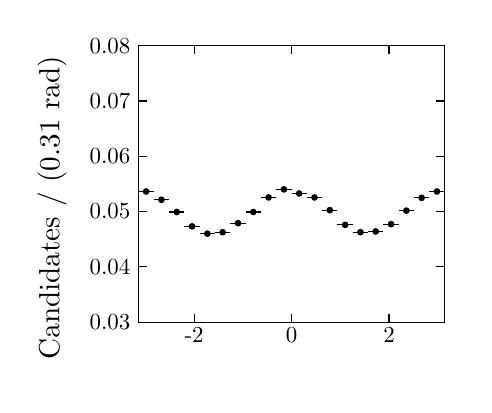
\begin{tikzpicture}
\pgfdeclareplotmark{cross} {
\pgfpathmoveto{\pgfpoint{-0.3\pgfplotmarksize}{\pgfplotmarksize}}
\pgfpathlineto{\pgfpoint{+0.3\pgfplotmarksize}{\pgfplotmarksize}}
\pgfpathlineto{\pgfpoint{+0.3\pgfplotmarksize}{0.3\pgfplotmarksize}}
\pgfpathlineto{\pgfpoint{+1\pgfplotmarksize}{0.3\pgfplotmarksize}}
\pgfpathlineto{\pgfpoint{+1\pgfplotmarksize}{-0.3\pgfplotmarksize}}
\pgfpathlineto{\pgfpoint{+0.3\pgfplotmarksize}{-0.3\pgfplotmarksize}}
\pgfpathlineto{\pgfpoint{+0.3\pgfplotmarksize}{-1.\pgfplotmarksize}}
\pgfpathlineto{\pgfpoint{-0.3\pgfplotmarksize}{-1.\pgfplotmarksize}}
\pgfpathlineto{\pgfpoint{-0.3\pgfplotmarksize}{-0.3\pgfplotmarksize}}
\pgfpathlineto{\pgfpoint{-1.\pgfplotmarksize}{-0.3\pgfplotmarksize}}
\pgfpathlineto{\pgfpoint{-1.\pgfplotmarksize}{0.3\pgfplotmarksize}}
\pgfpathlineto{\pgfpoint{-0.3\pgfplotmarksize}{0.3\pgfplotmarksize}}
\pgfpathclose
\pgfusepathqstroke
}
\pgfdeclareplotmark{cross*} {
\pgfpathmoveto{\pgfpoint{-0.3\pgfplotmarksize}{\pgfplotmarksize}}
\pgfpathlineto{\pgfpoint{+0.3\pgfplotmarksize}{\pgfplotmarksize}}
\pgfpathlineto{\pgfpoint{+0.3\pgfplotmarksize}{0.3\pgfplotmarksize}}
\pgfpathlineto{\pgfpoint{+1\pgfplotmarksize}{0.3\pgfplotmarksize}}
\pgfpathlineto{\pgfpoint{+1\pgfplotmarksize}{-0.3\pgfplotmarksize}}
\pgfpathlineto{\pgfpoint{+0.3\pgfplotmarksize}{-0.3\pgfplotmarksize}}
\pgfpathlineto{\pgfpoint{+0.3\pgfplotmarksize}{-1.\pgfplotmarksize}}
\pgfpathlineto{\pgfpoint{-0.3\pgfplotmarksize}{-1.\pgfplotmarksize}}
\pgfpathlineto{\pgfpoint{-0.3\pgfplotmarksize}{-0.3\pgfplotmarksize}}
\pgfpathlineto{\pgfpoint{-1.\pgfplotmarksize}{-0.3\pgfplotmarksize}}
\pgfpathlineto{\pgfpoint{-1.\pgfplotmarksize}{0.3\pgfplotmarksize}}
\pgfpathlineto{\pgfpoint{-0.3\pgfplotmarksize}{0.3\pgfplotmarksize}}
\pgfpathclose
\pgfusepathqfillstroke
}
\pgfdeclareplotmark{newstar} {
\pgfpathmoveto{\pgfqpoint{0pt}{\pgfplotmarksize}}
\pgfpathlineto{\pgfqpointpolar{44}{0.5\pgfplotmarksize}}
\pgfpathlineto{\pgfqpointpolar{18}{\pgfplotmarksize}}
\pgfpathlineto{\pgfqpointpolar{-20}{0.5\pgfplotmarksize}}
\pgfpathlineto{\pgfqpointpolar{-54}{\pgfplotmarksize}}
\pgfpathlineto{\pgfqpointpolar{-90}{0.5\pgfplotmarksize}}
\pgfpathlineto{\pgfqpointpolar{234}{\pgfplotmarksize}}
\pgfpathlineto{\pgfqpointpolar{198}{0.5\pgfplotmarksize}}
\pgfpathlineto{\pgfqpointpolar{162}{\pgfplotmarksize}}
\pgfpathlineto{\pgfqpointpolar{134}{0.5\pgfplotmarksize}}
\pgfpathclose
\pgfusepathqstroke
}
\pgfdeclareplotmark{newstar*} {
\pgfpathmoveto{\pgfqpoint{0pt}{\pgfplotmarksize}}
\pgfpathlineto{\pgfqpointpolar{44}{0.5\pgfplotmarksize}}
\pgfpathlineto{\pgfqpointpolar{18}{\pgfplotmarksize}}
\pgfpathlineto{\pgfqpointpolar{-20}{0.5\pgfplotmarksize}}
\pgfpathlineto{\pgfqpointpolar{-54}{\pgfplotmarksize}}
\pgfpathlineto{\pgfqpointpolar{-90}{0.5\pgfplotmarksize}}
\pgfpathlineto{\pgfqpointpolar{234}{\pgfplotmarksize}}
\pgfpathlineto{\pgfqpointpolar{198}{0.5\pgfplotmarksize}}
\pgfpathlineto{\pgfqpointpolar{162}{\pgfplotmarksize}}
\pgfpathlineto{\pgfqpointpolar{134}{0.5\pgfplotmarksize}}
\pgfpathclose
\pgfusepathqfillstroke
}
\definecolor{c}{rgb}{1,1,1};
\draw [color=c, fill=c] (5.1,4.72095) rectangle (9.9,9.16419);
\draw [color=c, fill=c] (5.772,5.43186) rectangle (9.66,8.94203);
\definecolor{c}{rgb}{0,0,0};
\draw [c] (5.772,5.43186) -- (5.772,8.94203) -- (9.66,8.94203) -- (9.66,5.43186) -- (5.772,5.43186);
\draw [c,line width=0.4] (5.8692,7.075) -- (5.8692,7.09126);
\draw [c,line width=0.4] (5.8692,7.09126) -- (5.8692,7.10752);
\draw [c,line width=0.4] (5.772,7.09126) -- (5.8692,7.09126);
\draw [c,line width=0.4] (5.8692,7.09126) -- (5.9664,7.09126);
\foreach \P in {(5.8692,7.09126)}{\draw[mark options={color=c,fill=c},mark size=1.201201pt,mark=*,mark size=1pt] plot coordinates {\P};}
\draw [c,line width=0.4] (6.0636,6.96943) -- (6.0636,6.98546);
\draw [c,line width=0.4] (6.0636,6.98546) -- (6.0636,7.00149);
\draw [c,line width=0.4] (5.9664,6.98546) -- (6.0636,6.98546);
\draw [c,line width=0.4] (6.0636,6.98546) -- (6.1608,6.98546);
\foreach \P in {(6.0636,6.98546)}{\draw[mark options={color=c,fill=c},mark size=1.201201pt,mark=*,mark size=1pt] plot coordinates {\P};}
\draw [c,line width=0.4] (6.258,6.81498) -- (6.258,6.83066);
\draw [c,line width=0.4] (6.258,6.83066) -- (6.258,6.84635);
\draw [c,line width=0.4] (6.1608,6.83066) -- (6.258,6.83066);
\draw [c,line width=0.4] (6.258,6.83066) -- (6.3552,6.83066);
\foreach \P in {(6.258,6.83066)}{\draw[mark options={color=c,fill=c},mark size=1.201201pt,mark=*,mark size=1pt] plot coordinates {\P};}
\draw [c,line width=0.4] (6.4524,6.63237) -- (6.4524,6.64764);
\draw [c,line width=0.4] (6.4524,6.64764) -- (6.4524,6.66292);
\draw [c,line width=0.4] (6.3552,6.64764) -- (6.4524,6.64764);
\draw [c,line width=0.4] (6.4524,6.64764) -- (6.5496,6.64764);
\foreach \P in {(6.4524,6.64764)}{\draw[mark options={color=c,fill=c},mark size=1.201201pt,mark=*,mark size=1pt] plot coordinates {\P};}
\draw [c,line width=0.4] (6.6468,6.53964) -- (6.6468,6.5547);
\draw [c,line width=0.4] (6.6468,6.5547) -- (6.6468,6.56975);
\draw [c,line width=0.4] (6.5496,6.5547) -- (6.6468,6.5547);
\draw [c,line width=0.4] (6.6468,6.5547) -- (6.744,6.5547);
\foreach \P in {(6.6468,6.5547)}{\draw[mark options={color=c,fill=c},mark size=1.201201pt,mark=*,mark size=1pt] plot coordinates {\P};}
\draw [c,line width=0.4] (6.8412,6.55841) -- (6.8412,6.57351);
\draw [c,line width=0.4] (6.8412,6.57351) -- (6.8412,6.58861);
\draw [c,line width=0.4] (6.744,6.57351) -- (6.8412,6.57351);
\draw [c,line width=0.4] (6.8412,6.57351) -- (6.9384,6.57351);
\foreach \P in {(6.8412,6.57351)}{\draw[mark options={color=c,fill=c},mark size=1.201201pt,mark=*,mark size=1pt] plot coordinates {\P};}
\draw [c,line width=0.4] (7.0356,6.67279) -- (7.0356,6.68815);
\draw [c,line width=0.4] (7.0356,6.68815) -- (7.0356,6.70352);
\draw [c,line width=0.4] (6.9384,6.68815) -- (7.0356,6.68815);
\draw [c,line width=0.4] (7.0356,6.68815) -- (7.1328,6.68815);
\foreach \P in {(7.0356,6.68815)}{\draw[mark options={color=c,fill=c},mark size=1.201201pt,mark=*,mark size=1pt] plot coordinates {\P};}
\draw [c,line width=0.4] (7.23,6.81512) -- (7.23,6.8308);
\draw [c,line width=0.4] (7.23,6.8308) -- (7.23,6.84649);
\draw [c,line width=0.4] (7.1328,6.8308) -- (7.23,6.8308);
\draw [c,line width=0.4] (7.23,6.8308) -- (7.3272,6.8308);
\foreach \P in {(7.23,6.8308)}{\draw[mark options={color=c,fill=c},mark size=1.201201pt,mark=*,mark size=1pt] plot coordinates {\P};}
\draw [c,line width=0.4] (7.4244,6.99956) -- (7.4244,7.01565);
\draw [c,line width=0.4] (7.4244,7.01565) -- (7.4244,7.03174);
\draw [c,line width=0.4] (7.3272,7.01565) -- (7.4244,7.01565);
\draw [c,line width=0.4] (7.4244,7.01565) -- (7.5216,7.01565);
\foreach \P in {(7.4244,7.01565)}{\draw[mark options={color=c,fill=c},mark size=1.201201pt,mark=*,mark size=1pt] plot coordinates {\P};}
\draw [c,line width=0.4] (7.6188,7.10127) -- (7.6188,7.11759);
\draw [c,line width=0.4] (7.6188,7.11759) -- (7.6188,7.1339);
\draw [c,line width=0.4] (7.5216,7.11759) -- (7.6188,7.11759);
\draw [c,line width=0.4] (7.6188,7.11759) -- (7.716,7.11759);
\foreach \P in {(7.6188,7.11759)}{\draw[mark options={color=c,fill=c},mark size=1.201201pt,mark=*,mark size=1pt] plot coordinates {\P};}
\draw [c,line width=0.4] (7.8132,7.04922) -- (7.8132,7.06542);
\draw [c,line width=0.4] (7.8132,7.06542) -- (7.8132,7.08163);
\draw [c,line width=0.4] (7.716,7.06542) -- (7.8132,7.06542);
\draw [c,line width=0.4] (7.8132,7.06542) -- (7.9104,7.06542);
\foreach \P in {(7.8132,7.06542)}{\draw[mark options={color=c,fill=c},mark size=1.201201pt,mark=*,mark size=1pt] plot coordinates {\P};}
\draw [c,line width=0.4] (8.0076,6.99899) -- (8.0076,7.01509);
\draw [c,line width=0.4] (8.0076,7.01509) -- (8.0076,7.03118);
\draw [c,line width=0.4] (7.9104,7.01509) -- (8.0076,7.01509);
\draw [c,line width=0.4] (8.0076,7.01509) -- (8.1048,7.01509);
\foreach \P in {(8.0076,7.01509)}{\draw[mark options={color=c,fill=c},mark size=1.201201pt,mark=*,mark size=1pt] plot coordinates {\P};}
\draw [c,line width=0.4] (8.202,6.83795) -- (8.202,6.85369);
\draw [c,line width=0.4] (8.202,6.85369) -- (8.202,6.86943);
\draw [c,line width=0.4] (8.1048,6.85369) -- (8.202,6.85369);
\draw [c,line width=0.4] (8.202,6.85369) -- (8.2992,6.85369);
\foreach \P in {(8.202,6.85369)}{\draw[mark options={color=c,fill=c},mark size=1.201201pt,mark=*,mark size=1pt] plot coordinates {\P};}
\draw [c,line width=0.4] (8.3964,6.65142) -- (8.3964,6.66674);
\draw [c,line width=0.4] (8.3964,6.66674) -- (8.3964,6.68205);
\draw [c,line width=0.4] (8.2992,6.66674) -- (8.3964,6.66674);
\draw [c,line width=0.4] (8.3964,6.66674) -- (8.4936,6.66674);
\foreach \P in {(8.3964,6.66674)}{\draw[mark options={color=c,fill=c},mark size=1.201201pt,mark=*,mark size=1pt] plot coordinates {\P};}
\draw [c,line width=0.4] (8.5908,6.55932) -- (8.5908,6.57442);
\draw [c,line width=0.4] (8.5908,6.57442) -- (8.5908,6.58952);
\draw [c,line width=0.4] (8.4936,6.57442) -- (8.5908,6.57442);
\draw [c,line width=0.4] (8.5908,6.57442) -- (8.688,6.57442);
\foreach \P in {(8.5908,6.57442)}{\draw[mark options={color=c,fill=c},mark size=1.201201pt,mark=*,mark size=1pt] plot coordinates {\P};}
\draw [c,line width=0.4] (8.7852,6.56836) -- (8.7852,6.58348);
\draw [c,line width=0.4] (8.7852,6.58348) -- (8.7852,6.5986);
\draw [c,line width=0.4] (8.688,6.58348) -- (8.7852,6.58348);
\draw [c,line width=0.4] (8.7852,6.58348) -- (8.8824,6.58348);
\foreach \P in {(8.7852,6.58348)}{\draw[mark options={color=c,fill=c},mark size=1.201201pt,mark=*,mark size=1pt] plot coordinates {\P};}
\draw [c,line width=0.4] (8.9796,6.66046) -- (8.9796,6.6758);
\draw [c,line width=0.4] (8.9796,6.6758) -- (8.9796,6.69113);
\draw [c,line width=0.4] (8.8824,6.6758) -- (8.9796,6.6758);
\draw [c,line width=0.4] (8.9796,6.6758) -- (9.0768,6.6758);
\foreach \P in {(8.9796,6.6758)}{\draw[mark options={color=c,fill=c},mark size=1.201201pt,mark=*,mark size=1pt] plot coordinates {\P};}
\draw [c,line width=0.4] (9.174,6.83165) -- (9.174,6.84737);
\draw [c,line width=0.4] (9.174,6.84737) -- (9.174,6.8631);
\draw [c,line width=0.4] (9.0768,6.84737) -- (9.174,6.84737);
\draw [c,line width=0.4] (9.174,6.84737) -- (9.2712,6.84737);
\foreach \P in {(9.174,6.84737)}{\draw[mark options={color=c,fill=c},mark size=1.201201pt,mark=*,mark size=1pt] plot coordinates {\P};}
\draw [c,line width=0.4] (9.3684,6.99409) -- (9.3684,7.01017);
\draw [c,line width=0.4] (9.3684,7.01017) -- (9.3684,7.02626);
\draw [c,line width=0.4] (9.2712,7.01017) -- (9.3684,7.01017);
\draw [c,line width=0.4] (9.3684,7.01017) -- (9.4656,7.01017);
\foreach \P in {(9.3684,7.01017)}{\draw[mark options={color=c,fill=c},mark size=1.201201pt,mark=*,mark size=1pt] plot coordinates {\P};}
\draw [c,line width=0.4] (9.5628,7.07472) -- (9.5628,7.09098);
\draw [c,line width=0.4] (9.5628,7.09098) -- (9.5628,7.10724);
\draw [c,line width=0.4] (9.4656,7.09098) -- (9.5628,7.09098);
\draw [c,line width=0.4] (9.5628,7.09098) -- (9.66,7.09098);
\foreach \P in {(9.5628,7.09098)}{\draw[mark options={color=c,fill=c},mark size=1.201201pt,mark=*,mark size=1pt] plot coordinates {\P};}
\draw [c,line width=0.4] (5.772,5.43186) -- (9.66,5.43186);
\draw [anchor= east] (9.66,4.78493) node[scale=1.28062, rotate=0]{$\phihel$};
\draw [c,line width=0.4] (6.47841,5.53984) -- (6.47841,5.43186);
\draw [c,line width=0.4] (7.716,5.53984) -- (7.716,5.43186);
\draw [c,line width=0.4] (8.95359,5.53984) -- (8.95359,5.43186);
\draw [c,line width=0.4] (6.47841,5.53984) -- (6.47841,5.43186);
\draw [c,line width=0.4] (8.95359,5.53984) -- (8.95359,5.43186);
\draw [anchor=base] (6.47841,5.17416) node[scale=0.828637, rotate=0]{-2};
\draw [anchor=base] (7.716,5.17416) node[scale=0.828637, rotate=0]{0};
\draw [anchor=base] (8.95359,5.17416) node[scale=0.828637, rotate=0]{2};
\draw [c,line width=0.4] (5.772,8.94203) -- (9.66,8.94203);
\draw [c,line width=0.4] (6.47841,8.83406) -- (6.47841,8.94203);
\draw [c,line width=0.4] (7.716,8.83406) -- (7.716,8.94203);
\draw [c,line width=0.4] (8.95359,8.83406) -- (8.95359,8.94203);
\draw [c,line width=0.4] (6.47841,8.83406) -- (6.47841,8.94203);
\draw [c,line width=0.4] (8.95359,8.83406) -- (8.95359,8.94203);
\draw [c,line width=0.4] (5.772,5.43186) -- (5.772,8.94203);
\draw [anchor= east] (4.67376,8.94203) node[scale=1.05463, rotate=90]{Candidates / (0.31 rad)};
\draw [c,line width=0.4] (5.88576,5.43186) -- (5.772,5.43186);
\draw [c,line width=0.4] (5.88576,6.1339) -- (5.772,6.1339);
\draw [c,line width=0.4] (5.88576,6.83593) -- (5.772,6.83593);
\draw [c,line width=0.4] (5.88576,7.53796) -- (5.772,7.53796);
\draw [c,line width=0.4] (5.88576,8.24) -- (5.772,8.24);
\draw [c,line width=0.4] (5.88576,8.94203) -- (5.772,8.94203);
\draw [anchor= east] (5.772,5.43186) node[scale=0.828637, rotate=0]{0.03};
\draw [anchor= east] (5.772,6.1339) node[scale=0.828637, rotate=0]{0.04};
\draw [anchor= east] (5.772,6.83593) node[scale=0.828637, rotate=0]{0.05};
\draw [anchor= east] (5.772,7.53796) node[scale=0.828637, rotate=0]{0.06};
\draw [anchor= east] (5.772,8.24) node[scale=0.828637, rotate=0]{0.07};
\draw [anchor= east] (5.772,8.94203) node[scale=0.828637, rotate=0]{0.08};
\draw [c,line width=0.4] (9.66,5.43186) -- (9.66,8.94203);
\draw [c,line width=0.4] (9.54624,5.43186) -- (9.66,5.43186);
\draw [c,line width=0.4] (9.54624,6.1339) -- (9.66,6.1339);
\draw [c,line width=0.4] (9.54624,6.83593) -- (9.66,6.83593);
\draw [c,line width=0.4] (9.54624,7.53796) -- (9.66,7.53796);
\draw [c,line width=0.4] (9.54624,8.24) -- (9.66,8.24);
\draw [c,line width=0.4] (9.54624,8.94203) -- (9.66,8.94203);
\end{tikzpicture}
